%%%%%%%%%%%%%%%%%%%%%%%%%%%%%%%%%%%%%%%%%
% Minimalist Book Title Page 
% LaTeX Template
% Version 1.0 (27/12/12)
%
% This template has been downloaded from:
% http://www.LaTeXTemplates.com
%
% Original author:
% Peter Wilson (herries.press@earthlink.net)
%
% License:
% CC BY-NC-SA 3.0 (http://creativecommons.org/licenses/by-nc-sa/3.0/)
% 
% Instructions for using this template:
% This title page compiles as is. If you wish to include this title page in 
% another document, you will need to copy everything before 
% \begin{document} into the preamble of your document. The title page is
% then included using \titleTH within your document.
%
%%%%%%%%%%%%%%%%%%%%%%%%%%%%%%%%%%%%%%%%%

%----------------------------------------------------------------------------------------
%	PACKAGES AND OTHER DOCUMENT CONFIGURATIONS
%----------------------------------------------------------------------------------------

%\title{Microprocessor Architecture : Labo 1}

\documentclass{article}

\usepackage[utf8]{inputenc}
\usepackage[T1]{fontenc}
\usepackage[svgnames]{xcolor} % Required to specify font color
\usepackage{mathpazo}
\usepackage{floatrow}
\usepackage{geometry}%réglages mise en page
\geometry{%
a4paper, % note : l'option a4paper tuait la marge supérieure.
body={170mm,250mm}, %
left=25mm,top=25mm,right=25mm, %
headheight=21mm,headsep=7mm,
marginparsep=4mm,
marginparwidth=20mm, %
footnotesep=50mm
}
\usepackage{longtable}
\usepackage{pdflscape}
% allows for temporary adjustment of side margins
\usepackage{chngpage}
\usepackage{graphicx}
\usepackage{float}
\usepackage{color}
\usepackage{amssymb}

\definecolor{pblue}{rgb}{0.13,0.13,1}
\definecolor{pgreen}{rgb}{0,0.5,0}
\definecolor{pred}{rgb}{0.9,0,0}
\definecolor{pgrey}{rgb}{0.46,0.45,0.48}

\usepackage{listings}
\lstset{ % 
  language=R,                % the language of the code 
  basicstyle=\footnotesize,           % the size of the fonts that are used for the code 
  numbers=left,                   % where to put the line-numbers 
  numberstyle=\tiny\color{gray},  % the style that is used for the line-numbers 
  stepnumber=2,                   % the step between two line-numbers. If it's 1, each line 
                                  % will be numbered 
  numbersep=5pt,                  % how far the line-numbers are from the code 
  backgroundcolor=\color{white},      % choose the background color. You must add \usepackage{color} 
  showspaces=false,               % show spaces adding particular underscores 
  showstringspaces=false,         % underline spaces within strings 
  showtabs=false,                 % show tabs within strings adding particular underscores 
  frame=single,                   % adds a frame around the code 
  rulecolor=\color{black},        % if not set, the frame-color may be changed on line-breaks within not-black text (e.g. commens (green here)) 
  tabsize=2,                      % sets default tabsize to 2 spaces 
  captionpos=b,                   % sets the caption-position to bottom 
  breaklines=true,                % sets automatic line breaking 
  breakatwhitespace=false,        % sets if automatic breaks should only happen at whitespace 
  %title=\lstname,                   % show the filename of files included with \lstinputlisting; 
                                  % also try caption instead of title 
  keywordstyle=\color{blue},          % keyword style 
  commentstyle=\color{dkgreen},       % comment style 
  stringstyle=\color{purple},         % string literal style 
  escapeinside={\%*}{*)},            % if you want to add a comment within your code 
  morekeywords={*,...}               % if you want to add more keywords to the set 
} 
\usepackage{amssymb}
\usepackage[boxed]{algorithm2e}
\usepackage{array}

\newcommand*{\course}{\fbox{INFO-H-413}} % Generic publisher logo

%----------------------------------------------------------------------------------------
%	TITLE PAGE
%----------------------------------------------------------------------------------------

\newcommand*{\titleTH}{\begingroup % Create the command for including the title page in the document
\raggedleft % Right-align all text
\vspace*{\baselineskip} % Whitespace at the top of the page

{\Large \textsc{Anthony Debruyn}}\\[0.167\textheight] % Author name

{\LARGE\bfseries Heuristic Optimisation}\\[\baselineskip] % First part of the title, if it is unimportant consider making the font size smaller to accentuate the main title

{\textcolor{Orange}{\Huge Implementation Exercise 2}}\\[\baselineskip] % Main title which draws the focus of the reader

{\Large \textit{Stochastic local search algorithms for the PFSP}}\par % Tagline or further description

\vfill % Whitespace between the title block and the publisher

%\vspace*{30\baselineskip} % Whitespace at the bottom of the page

{\large Dr. F. Mascia, Dr. T. Stützle \course}\par % Publisher and logo

%\vspace*{5\baselineskip} % Whitespace at the bottom of the page
\endgroup}

%----------------------------------------------------------------------------------------
%	BLANK DOCUMENT
%----------------------------------------------------------------------------------------

\begin{document} 

\thispagestyle{empty}

\titleTH % This command includes the title page

\newpage
\section{Introduction}
The goal of this project was to implement 2 SLS algorithms, and analyse and compare them by means of statistical tests, run-time distributions and correlation plots. 

\section{Studied SLS Algorithms}
\subsection{Simulated Annealing}
The first algorithm tested is the simulated annealing. Its pseudo code is the following:

\begin{algorithm}[H]
 Get initial solution $s$ with SLACK heuristic\;
 Set initial temperature $T$ to get 0.05 acceptance ratio\;
 $counter = 0$\;
 \While{Allowed run-time not elapsed}{
  Choose randomly a neighbour $s'$ of $s$ in the insertion neighbourhood\;
  \If{$s'$ satisfies the Metropolis condition}{
   $s := s'$\;
   }
   $counter = counter + 1$\;
   \If{$counter >= q * |N(s)|$}{
	$T = T*r$\;
	$counter = 0$\;
   }
 }
 \caption{Simulated Annealing}
\end{algorithm}

The values used for the parameters are listed here:
\begin{description}
\item[Initial acceptance ratio $F_0$ of $0.05$:] This value of the initial acceptance ratio was chosen from \emph{Kim YD, Lim HG, Park MW. Search heuristics for a flowshop scheduling problem in a printed circuit board assembly process. European Journal
of Operational Research 1996;91:124–43.}, an article referenced in \emph{Eva Vallada,Rubén Ruiz, Gerardo Minella. Minimising total tardiness in the m-machine flow-shop problem: A review and evaluation of heuristics and metaheuristics. Computers \& OR, 35(4):1350–1373, 2008.} put in the guidelines. The value was the best tested one.

\item[$q$:] This factor is found in the epoch length, and its value is 2. The epoch length is the number of steps made with the same temperature. It is proportional to the size of the neighbourhood, so the annealing schedule adapts to the size of the problem. Again, $q = 2$ was the best value tested in the above mentioned paper.

\item[$r$:] It is the factor used in the geometric cooling, and its value is 0.7, as in the article best algorithm.
\end{description}

The first solution of the algorithm is obtained with the SLACK heuristic, and the neighbourhood used is the insertion neighbourhood. These offered very good results in the first implementation exercise.\\

The first temperature is obtained by making a first exploration of the neighbourhood with the first solution, and taking the average cost increase in the worsening solutions only. This average was then used with the desired initial acceptance ratio to compute the initial temperature:

$$T_0 = \frac{-\overline{\Delta}}{\ln{F_0}}$$, with

$$\overline{\Delta} = \sum_{worsening ~solutions ~s'}{cost(s') - cost(s)}$$, where $s$ is the initial solution.\\

The termination condition is based on the run-time of the algorithm.\\

One improvement of the algorithm listed in the course was used, it is the 0.05 acceptance ratio. A low temperature start helps "prevent good initial candidate solutions from being too easily destroyed by worsening steps".

\subsection{Iterated Local Search}

The second algorithm is the hybrid iterated local search. Here is the pseudo code:

\begin{algorithm}[H]
 $s \leftarrow$ Get initial solution $s$ with SLACK heuristic\;
 $s \leftarrow$ Perform local search with $s$\;
 \While{Allowed run-time not elapsed}{
 	$s' \leftarrow$ Perturbation on $s$\;
 	$s' \leftarrow$ Perform local search with $s'$\;
 	\If{$cost(s') <= cost(s)$}{
 		$s := s'$\;
 	}
 }
 \caption{Iterated Local Search}
\end{algorithm}

As initial solution generator, the SLACK heuristic is again used, as it yielded good results in the previous implementation exercise.\\

As pivoting mode, the first pivoting mode is employed, taking the first improving solution of the neighbourhood.\\

The neighbourhood generator used is the insertion generator, taking a job and putting it at another place in the order of jobs.\\

The perturbation technique employed is an insertion perturbation of 4 consecutive insertions of a random job at a random place.\\

The acceptance criterion uses the cost of the solutions to take the new best permutation. It forces the solutions algorithm to keep the best solution at all times.\\

As we can see, this algorithm uses perturbation to escape from a local minimum each time one is encountered. This leads to a iteration through the set of local minima. If the run-time is long enough, this could theoretically yield very good results.\\

\section{Results}

\subsection{Mean Relative Percentage Deviations}

\begin{center}
\begin{figure}[H]
\begin{tabular}{| >{\centering\arraybackslash}m{2cm} | >{\centering\arraybackslash}m{2cm} | >{\centering\arraybackslash}m{2cm} |}
\hline
Instances & SA & ILS \\ \hline
100x20\_1	&	114	&	-3	\\ \hline
100x20\_10	&	122	&	-1	\\ \hline
100x20\_2	&	174	&	-1	\\ \hline
100x20\_3	&	106	&	-2	\\ \hline
100x20\_4	&	124	&	-1	\\ \hline
100x20\_5	&	135	&	-1	\\ \hline
100x20\_6	&	111	&	-2	\\ \hline
100x20\_7	&	111	&	-3	\\ \hline
100x20\_8	&	113	&	-1	\\ \hline
100x20\_9	&	101	&	-3	\\ \hline

\end{tabular}

\caption{100 jobs}
\end{figure}

\begin{figure}[H]
\begin{tabular}{| >{\centering\arraybackslash}m{2cm} | >{\centering\arraybackslash}m{2cm} | >{\centering\arraybackslash}m{2cm} |}
\hline
Instances & SA & ILS \\ \hline
50x20\_1	&	349	&	1	\\ \hline
50x20\_10	&	389	&	0	\\ \hline
50x20\_2	&	1052	&	-5	\\ \hline
50x20\_3	&	825	&	3	\\ \hline
50x20\_4	&	2081	&	9	\\ \hline
50x20\_5	&	760	&	2	\\ \hline
50x20\_6	&	527	&	0	\\ \hline
50x20\_7	&	718	&	0	\\ \hline
50x20\_8	&	232	&	0	\\ \hline
50x20\_9	&	557	&	0	\\ \hline

\end{tabular}

\caption{50 jobs}
\end{figure}

\begin{figure}[H]
\begin{tabular}{| >{\centering\arraybackslash}m{2cm} | >{\centering\arraybackslash}m{2cm} | >{\centering\arraybackslash}m{2cm} |}
\hline
Instances & SA & ILS \\ \hline
60x20\_1	&	250	&	0	\\ \hline
60x20\_10	&	275	&	0	\\ \hline
60x20\_2	&	182	&	-1	\\ \hline
60x20\_3	&	158	&	0	\\ \hline
60x20\_4	&	351	&	0	\\ \hline
60x20\_5	&	237	&	0	\\ \hline
60x20\_6	&	269	&	0	\\ \hline
60x20\_7	&	416	&	0	\\ \hline
60x20\_8	&	270	&	0	\\ \hline
60x20\_9	&	297	&	0	\\ \hline

\end{tabular}

\caption{60 jobs}
\end{figure}

\begin{figure}[H]
\begin{tabular}{| >{\centering\arraybackslash}m{2cm} | >{\centering\arraybackslash}m{2cm} | >{\centering\arraybackslash}m{2cm} |}
\hline
Instances & SA & ILS \\ \hline
70x20\_1	&	188	&	0	\\ \hline
70x20\_10	&	203	&	-1	\\ \hline
70x20\_2	&	154	&	0	\\ \hline
70x20\_3	&	242	&	0	\\ \hline
70x20\_4	&	260	&	0	\\ \hline
70x20\_5	&	214	&	0	\\ \hline
70x20\_6	&	240	&	0	\\ \hline
70x20\_7	&	213	&	0	\\ \hline
70x20\_8	&	245	&	-1	\\ \hline
70x20\_9	&	217	&	-1	\\ \hline

\end{tabular}

\caption{70 jobs}
\end{figure}

\begin{figure}[H]
\begin{tabular}{| >{\centering\arraybackslash}m{2cm} | >{\centering\arraybackslash}m{2cm} | >{\centering\arraybackslash}m{2cm} |}
\hline
Instances & SA & ILS \\ \hline
80x20\_1	&	192	&	0	\\ \hline
80x20\_10	&	167	&	-1	\\ \hline
80x20\_2	&	167	&	0	\\ \hline
80x20\_3	&	159	&	-2	\\ \hline
80x20\_4	&	180	&	0	\\ \hline
80x20\_5	&	134	&	0	\\ \hline
80x20\_6	&	168	&	-1	\\ \hline
80x20\_7	&	226	&	-2	\\ \hline
80x20\_8	&	130	&	0	\\ \hline
80x20\_9	&	224	&	-1	\\ \hline

\end{tabular}

\caption{80 jobs}
\end{figure}

\begin{figure}[H]
\begin{tabular}{| >{\centering\arraybackslash}m{2cm} | >{\centering\arraybackslash}m{2cm} | >{\centering\arraybackslash}m{2cm} |}
\hline
Instances & SA & ILS \\ \hline
90x20\_1	&	159	&	-1	\\ \hline
90x20\_10	&	119	&	-2	\\ \hline
90x20\_2	&	116	&	-1	\\ \hline
90x20\_3	&	132	&	-1	\\ \hline
90x20\_4	&	128	&	-2	\\ \hline
90x20\_5	&	172	&	0	\\ \hline
90x20\_6	&	124	&	0	\\ \hline
90x20\_7	&	151	&	-3	\\ \hline
90x20\_8	&	145	&	-2	\\ \hline
90x20\_9	&	119	&	-1	\\ \hline

\end{tabular}

\caption{90 jobs}
\end{figure}

\end{center}

As we can see on the figures above, the 2 algorithms offer very different results. The SA is the worst tested, if we also look back at the first implementation exercise. The ILS, on the other hand, is the best and yields solutions that are better than the best known. On average, the SA has a relative percentage deviation of 278, while the ILS one is 0.

\subsection{Correlation Plots of the Mean Relative Percentage Deviation}

\begin{figure}[H]
\centering 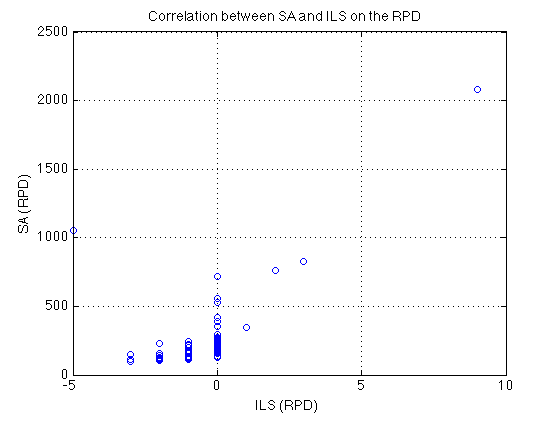
\includegraphics[width=\textwidth]{correlation.png}
\caption{Correlation between SA and ILS on the MRPD of each instance}
\end{figure}

Except the outlier on the upper left zone (above 1000), the graph shows a certain correlation between the 2 algorithms. The higher the MRPD on the ILS side the higher on the SA side. Moreover, the values are a lot more spread on the SA side. For the ILS, the values rarely go above 0.


\subsection{Statistical Test}

With the help of the Wilcoxon test, the p-value $1.670281*10^{-11}$ was obtained, confirming what the previous graph and tables were showing. The probability to incorrectly rejecting the hypothesis of similarity between the 2 algorithms is 1.670281e-11. So the 2 algorithms are, with a high probability very different.

\end{document}